\subsection{Эквивалентные преобразования электрических цепей}

Эквивалентные преобразования заключаются в замене некоторых участков цепи таким образом, что число выводов исходного участка соответствует числу выводов эквивалентного, и при подаче на соответствующие выводы равных потенциалов, через соответствующие узлы течет равный ток.

\begin{center}
	\begin{figure}[h!]
		\center{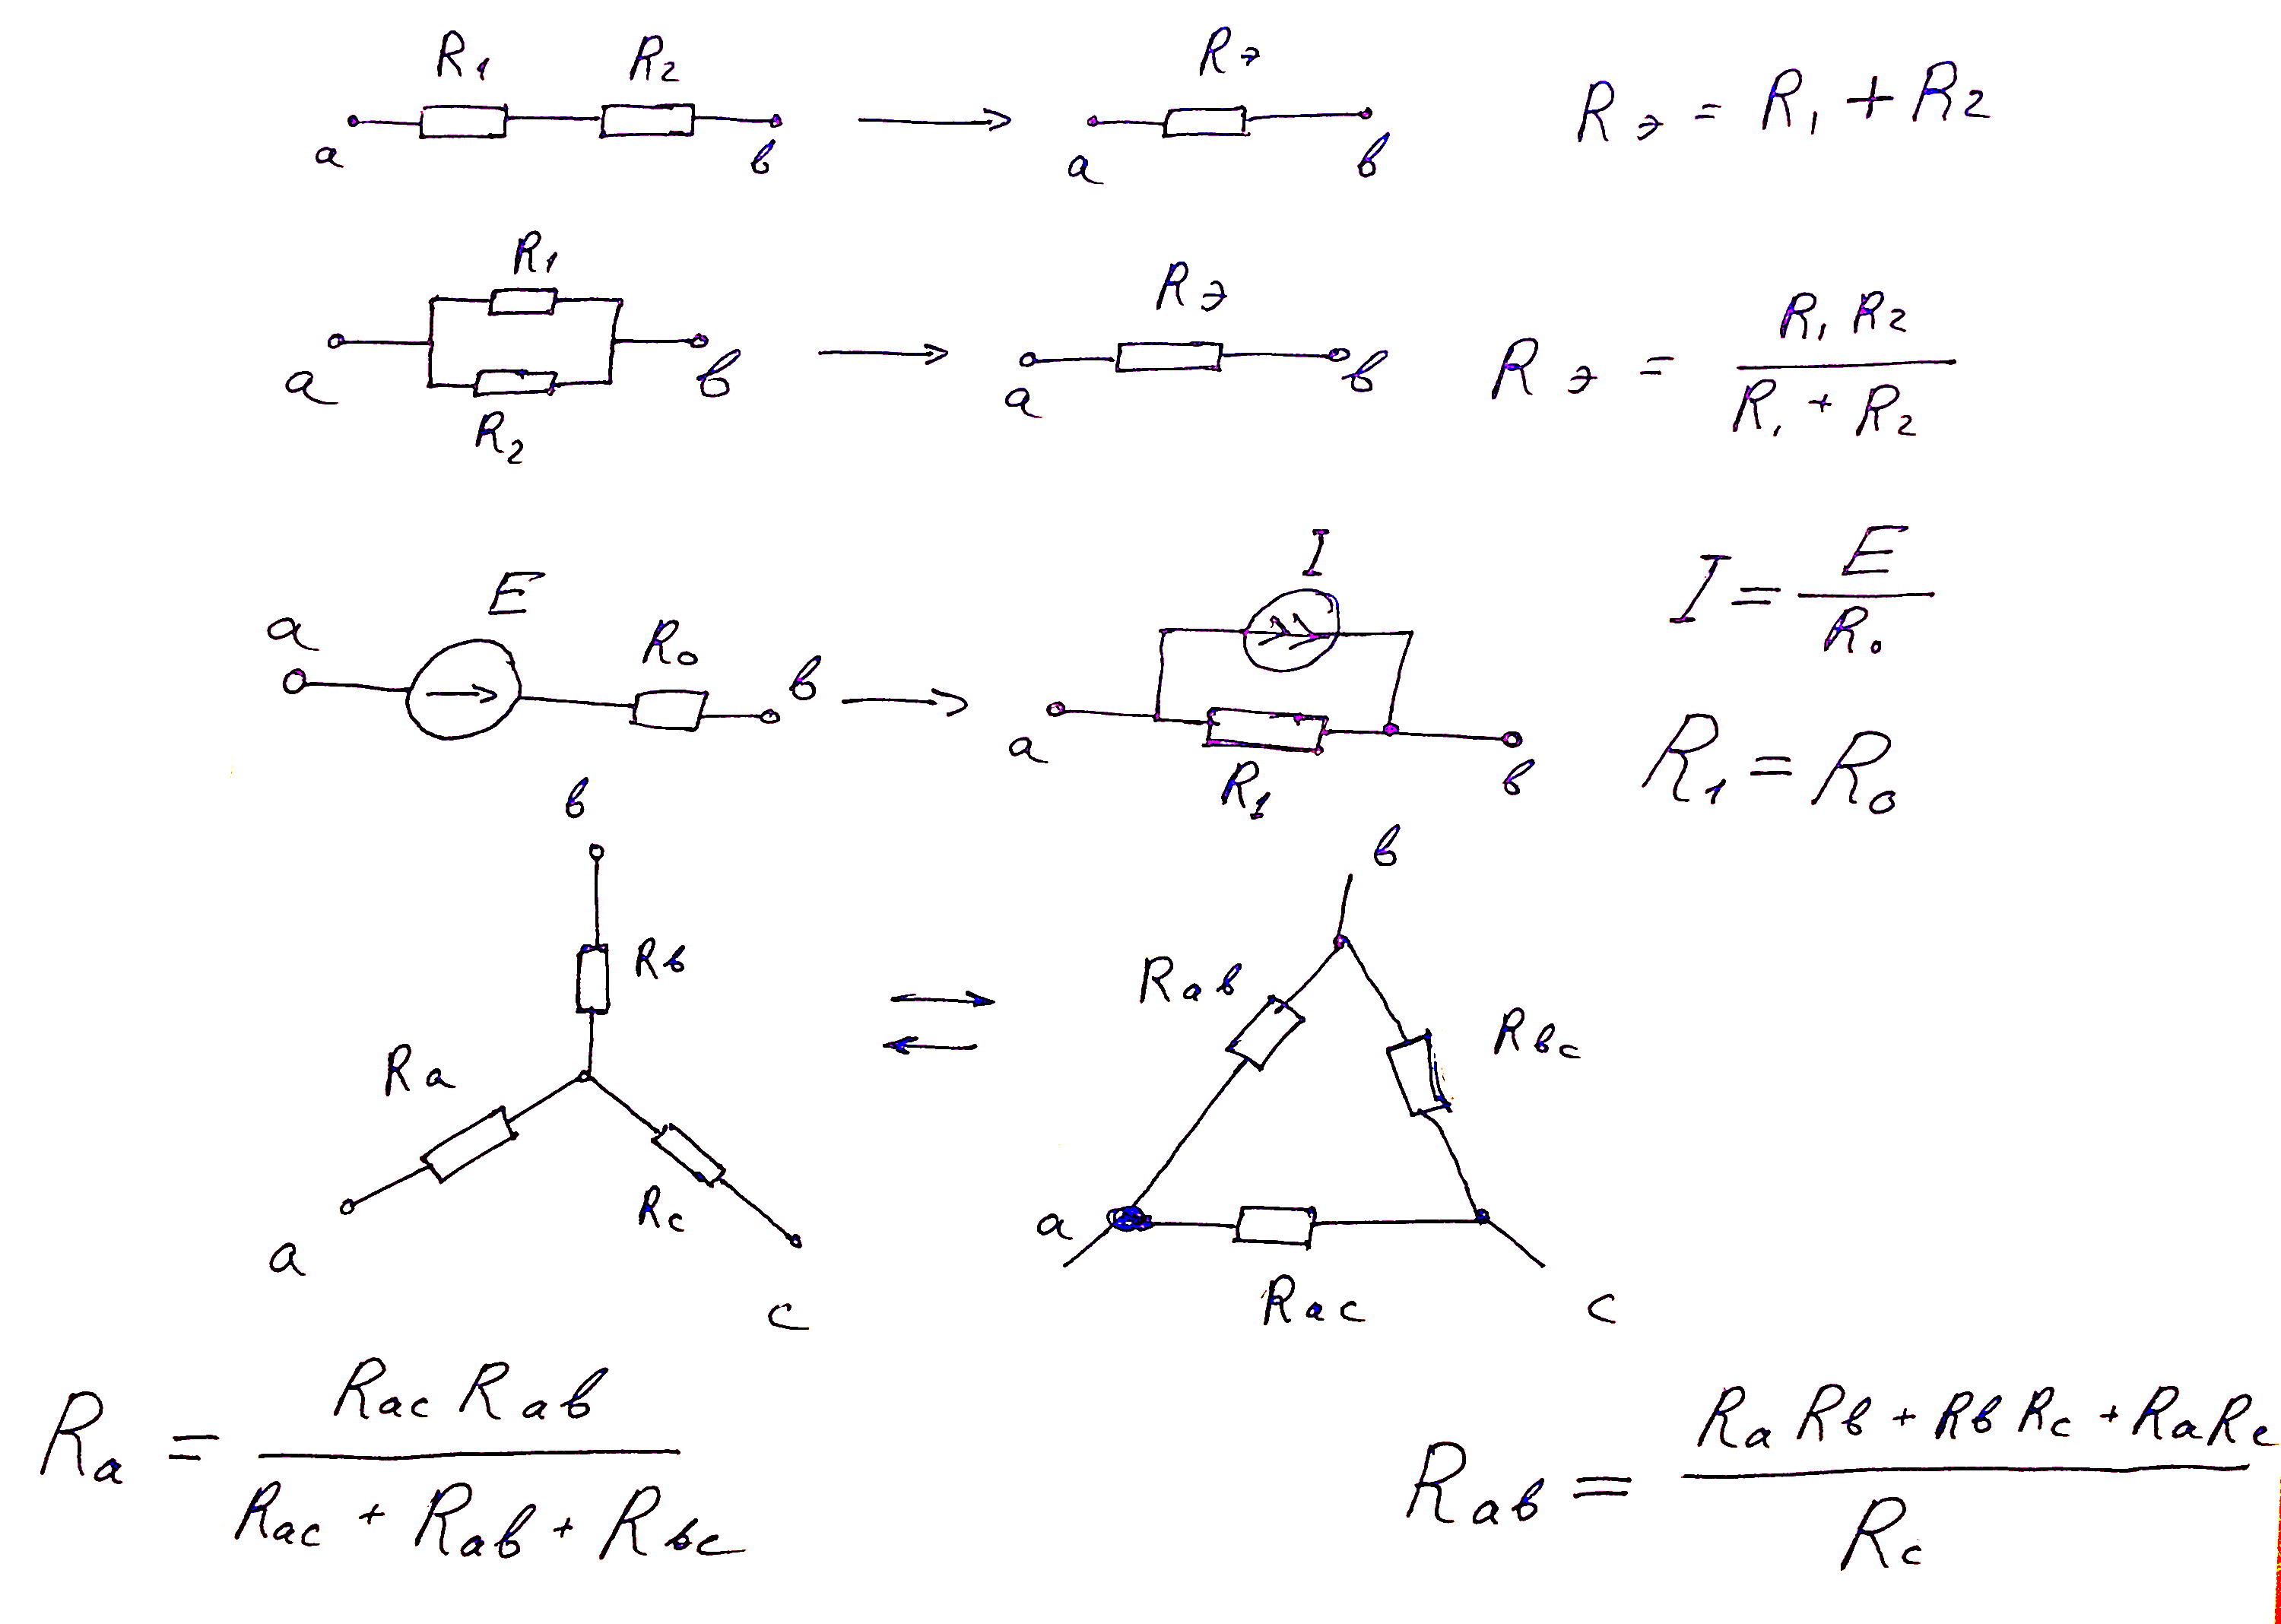
\includegraphics[scale=0.16]{transform.png}}
		\caption{преобразования}	
	\end{figure}
\end{center}	

\pagebreak